% LaTeX-Vorlage zur Erstellung einer Projektarbeit (Dokumentation eines Projekts)
% auf Basis der Vorlage für eine
% Abschlussarbeit in der Fakultät Elektrotechnik, Medien und Informatik an der OTH Amberg-Weiden
% Diese Vorlage entstand im Rahmen des Kurses "LaTeX fürs Studium"
% Aktuelle Version: v0.01
% Stand: 03.06.2023
%
% Changelog:
%
% v0.01: 03.06.2023, Anpassung der Vorlage für Projektarbeiten (article statt report, keine Titelblätter)
%
\documentclass[12pt,oneside]{article}
\usepackage[T1]{fontenc}		% Einstellungen fuer Umlaute usw.
\usepackage[utf8x]{inputenc}
\usepackage[ngerman]{babel}
\usepackage{tabularx}
\setcounter{secnumdepth}{5}
\setcounter{tocdepth}{3}

\usepackage{parskip}			% Einstellungen fuer Absaetze: Abstand statt Einrueckung
\usepackage{graphicx}			% Standard Bildeinbindungspaket

\usepackage[a4paper,			% Papierformat A4
	    left=2.5cm,				% linker Rand
	    right=2.5cm,			% rechter Rand
	    top=1.5cm,				% oberer Rand
	    bottom=1.5cm,			% unter Rand
	    marginparsep=5mm,		% Abstand der Randnotizen
	    marginparwidth=10mm, 	% Breite der Randnotizen
	    headheight=7mm,			% Hoehe der Kopfzeile
	    headsep=1.2cm,			% Abstand der Kopfzeile
	    footskip=1.5cm,			% Abstand der Fusszeile
	    includeheadfoot]{geometry}

\usepackage{fancyhdr}						% Konfiguration von Kopf- und Fusszeilen
\pagestyle{fancy}							% Seitenstil 'fancy'
\fancyhf{}									% vorhandene Einstellungen loeschen
\setlength{\headwidth}{\textwidth}			% Kopf- und Fusszeile so breit wie der Haupttext
\fancyfoot[R]{\thepage} 					% Festlegung des Seitenstils: Seitenzahlen in der Fusszeile rechts
\fancyfoot[L]{\IhreArbeit}					% Kapitelnr. und -Bezeichnung in der Fusszeile links
\fancyhead[L]{\IhreGruppe: \IhrVornameEins\ \IhrNachnameEins\ \& \IhrVornameZwei\ \IhrNachnameZwei}	% Vorname und Name in der Kopfzeile links
\renewcommand{\sectionmark}[1]{	    		% Definition der Ausgabe des Kapitels
  \markboth{Abschnitt \thesection. #1}{}}
\renewcommand{\headrulewidth}{0.5pt}		% Trennlinie zwischen Kopfzeile und Haupttext
\renewcommand{\footrulewidth}{0.5pt}		% Trennlinie zwischen Haupttext und Fusszeile
\fancypagestyle{plain}{				     	% Anpassung des Seitenstils 'plain' bei Beginn neuer Kapitel
  \fancyhf{}								% Vorbelegung loeschen
  \fancyfoot[C]{\thepage}					% Seitenzeilen in der Fusszeile mittig
}

%\usepackage{amsmath}			% Pakete fuer den Mathematikmodus
%\usepackage{amssymb}
%\usepackage[intlimits]{empheq}

\usepackage[sc]{mathpazo}		% Schriftart Palatino fuer Haupttext und Mathematikmodus
\usepackage{pifont}				% zusaetzliche Symbole

% \usepackage[format=hang,		% Einstellung fuer Bildunterschriften
            % font={footnotesize},
            % labelfont={bf},
            % margin=1cm,
            % aboveskip=5pt,
            % position=bottom]{caption}

\usepackage{graphicx}							% Einbinden von Graphiken
\usepackage[svgnames,cmyk,table,hyperref]{xcolor} 	% Verwendung von Farben

\definecolor{aoenglish}{rgb}{0.0, 0.5, 0.0}
\definecolor{battleshipgrey}{rgb}{0.52, 0.52, 0.51}
\definecolor{cardinal}{rgb}{0.77, 0.12, 0.23}


%\usepackage{tikz}								% Erstellen von Grafiken
%\usetikzlibrary{positioning,arrows,plotmarks} % TikZ-Bibliotheken
%\usepackage{pgfplots}                           % Darstellung von Plots, Funktionen, Graphen usw.

%
% Weitere Pakete
%
\usepackage{listings}			% Darstellung von Quellcode
\lstloadlanguages{[ISO]C++,Java,XML,[LaTeX]TeX}
\lstset{language=C++,
	numbers = none,
	basicstyle = \small\ttfamily,
	keywordstyle = \color{blue},
	commentstyle = \color{battleshipgrey},
	stringstyle = \color{cardinal},
	columns = flexible,
	showstringspaces = false
}
%

\lstdefinelanguage{JS}{
	keywords={typeof, new, true, false, catch, function, return, null, catch, switch, var, if, in, while, do, else, case, break},
	keywordstyle=\color{blue}\bfseries,
	ndkeywords={class, export, boolean, throw, implements, import, this},
	ndkeywordstyle=\color{blue}\bfseries,
	identifierstyle=\color{black},
	sensitive=false,
	comment=[l]{//},
	morecomment=[s]{/*}{*/},
	commentstyle=\color{battleshipgrey}\ttfamily,
	stringstyle=\color{cardinal}\ttfamily,
	morestring=[b]',
	morestring=[b]"
}

\usepackage[square,numbers,sort]{natbib} % Zitationsstil mit Attribut lastchecked
%
%\usepackage[european, siunitx]{circuitikz}	% Darstellung von Schaltungen
%
%\usepackage{enumerate}			% Formatierung nummerierter Listen

% 
% Persoenliche Angaben
% 
\newcommand*{\IhrVornameEins}{Johannes}
\newcommand*{\IhrNachnameEins}{Grosch}
\newcommand*{\IhrVornameZwei}{Daniel}
\newcommand*{\IhrNachnameZwei}{Hartl}
\newcommand*{\IhreGruppe}{Gruppe 42}
\newcommand*{\IhrStudiengang}{Industrie-4.0-Informatik}
\newcommand*{\IhreArbeit}{Projektarbeit Mobile \& Ubiquitous Computing SoSe 2024}
\newcommand*{\IhreSchluesselwoerter}{Android, ESP32, MQTT, IoT, Pulsoximeter, MAX30100, WLAN}
\newcommand*{\IhrErstpruefer}{Prof. Dr. Ulrich Schäfer}

\newcommand{\quoteM}[1]{\glqq {#1}\grqq{}}
\renewcommand{\lstlistlistingname}{Quellcodeverzeichnis}

\usepackage[bookmarks, raiselinks, pageanchor, % PDF-Einstellungen
            hyperindex, colorlinks,
            citecolor=black, linkcolor=black,
            urlcolor=black, filecolor=black,
            menucolor=black]{hyperref}
\hypersetup{pdftitle={\IhreArbeit},%
            pdfauthor={\IhrVornameEins\ \IhrNachnameEins{} \& \IhrVornameZwei\ \IhrNachnameZwei},%
            pdfsubject={\IhreGruppe},%
            pdfkeywords={\IhreSchluesselwoerter}}

%
% Beginn des Textteils
%

\begin{document}
  \thispagestyle{empty}
  \originalTeX
  \begin{center}
 	\Large
 	Ostbayerische Technische Hochschule Amberg-Weiden\\
 Fakultät Elektrotechnik, Medien und Informatik\\[.8cm]
 \large \IhrErstpruefer\\[.8cm]
 \Large \IhreArbeit\\[.8cm]
 \large \IhreGruppe: \IhrVornameEins\ \IhrNachnameEins\ \&
 \IhrVornameZwei\ \IhrNachnameZwei\\[.8cm]
 \large Studiengang \IhrStudiengang\\[.8cm]
 \today\\[2.5cm]
  \end{center}
  
  \tableofcontents

  \clearpage
  
  %
  % Einleitung
  %
  
  \section{Einleitung}
	Das Ziel des Projekts ist es, mittels des optische Herzfrequenzmess- und Pulsoximetriesensormoduls MAX30100\cite{max30100breakout} ein Puls- und Pulsoximetriemessgerät zu realisieren, welches über eine MQTT Broker Anbindung fähig ist Daten an eine Android Applikation zu übertragen.


  %
  % Projektplanung und Vorgehen
  %
  
  \section{Projektplanung und Vorgehen}
  \subsection{Planungsphase}
	\begin{figure}[tph!]
	 	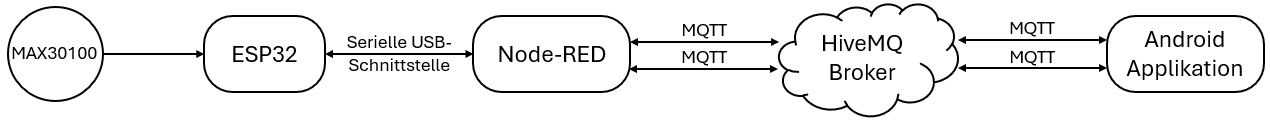
\includegraphics[width=0.9\textwidth]{kommunikationsdiagramm}
	 	\caption{Datenflussdiagramm innerhalb des Projekts}
	 	\label{fig:datadiagram}
	\end{figure}
	Die Planung ging nach dem Prinzip \quoteM{Divide et impera} Teile und herrsche von Statten. Da in dem System so viele separate Komponenten, die bis auf die ein- und ausgehenden Werte autonom voneinander sind. Diesen, bzw. dem Format, in dem diese zwischen den Komponenten übertragen werden ist das Unterkapitel \ref{subsec:internalCommunication} gewidmet.\par
	Die Arbeitsaufteilung wurde derartig vorgenommen, dass Herr Grosch die Android Applikation, was wir als das umfangreichste Subsystem realisiert haben und Herr Hartl die zwei kleineren Subsysteme und die \LaTeX{} Dokumentation erstellt, da er bereits versiert mit \LaTeX{} ist.
  \subsection{Vorgehen}
	Zur Realisierung haben wir uns an einen inkrementellen Ansatz gehalten. So haben wir zuerst die Datenquelle, die angepasste MAX30100 Bibliothek entwickelt und uns bildhaft in Abbildung \ref{fig:datadiagram} nach rechts vorgearbeitet. So konnte das, in der Entwicklung befindliche System jederzeit mit realen Daten getestet werden und es bestand kein Bedarf an Testdatensätzen o.ä.\par
	Dieser Entwicklungsansatz wird ebenfalls in der Struktur des Kapitels \ref{sec:implementation} wiedergegeben.
  \subsection{Kommunikation zwischen Komponenten}
	\label{subsec:internalCommunication}
	Die Serielle Kommunikation zwischen dem ESP\_32 und dem Laptop ist mit 10Hz auf 115200 Baud realisiert. Um unnötigen Overhead zu vermeiden findet sie in folgender, minimalistischer Synthax statt:\par
	\textbf{<Pulsschlag>;<Sauerstoffsättigung>}\par
	Diese Telegramme werden dann in Node-RED\cite{nodeRED} eine Sekunde bzw. zehn Nachrichten lang gesammelt, nach Parametern aufgedröselt, je ein Durchschnitt gebildet um den Jitter zu verringern und die Graphen zu glätten und dann an den HiveMQ Broker\cite{hiveMQ} zu senden, wo es unter dem Topic \textbf{afkdcdjkcnks/sensor/data/raw/sensor} für die Sensordaten der App zugänglich gemacht werden.\par
	Andersherum published die Android Applikation unter dem Topic \textbf{afkdcdjkcnks/sensor/ctrl/raw/sensor} die zuletzt ausgewählte View, nach der die Node-RED Logik die zu publishenden Daten auswählt.
  
  
  
  
  %
  % Implementierung
  %
  
  \section{Implementierung}
  \label{sec:implementation}
  
  Der ESP\_32\cite{esp32} ist wie in folgender Abbildung gezeigt mit dem MAX30100\cite{max30100breakout} verbunden. 
  \begin{figure}[tph!]
  	\begin{center}
  		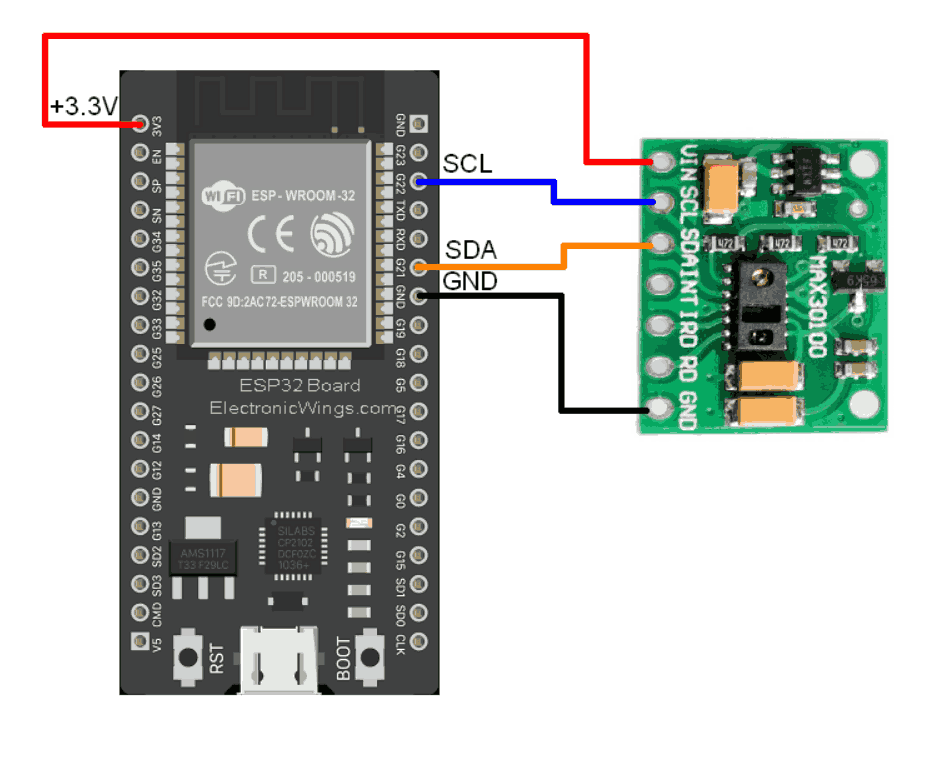
\includegraphics[width=0.5\textwidth]{MAX30100 Interfacing ESP32}
	  	\caption{Verkabelung des ESP\_32 mit dem MAX30100\cite{max30100tutorial}}
	  	\label{fig:espSchaltung}
  	\end{center}
  \end{figure}
Diese Konfiguration ist von der Website Electronicwings.com übernommen.
  \begin{itemize}
  	\item 3,3V $\longleftrightarrow$ VIN
  	\item G22 $\longleftrightarrow$ SCL
  	\item G21 $\longleftrightarrow$ SDA
  	\item GND $\longleftrightarrow$ GND
  \end{itemize}
  
  
  \subsection{Änderungen an der MAX30100 Bibliothek}
  \quoteM{[Der] MAX30100 ist ein optisches Herzfrequenzmess- und Pulsoximetriesensormodul. Es
  integriert zwei LEDs (IR und Rot), einen Photodetektor (Rot), eine optimierte Optik
  und eine rauscharme analoge Signalverarbeitung zur Erkennung von Pulsoximetrie-
  und Herzfrequenzsignalen. Das Signal wird von einer rauscharmen analogen
  Signalverarbeitungseinheit verarbeitet und über die I2C-Schnittstelle an die
  Ziel-MCU weitergeleitet.}\cite{max30100breakout}\par
  Die Basis zum Betreiben des MAX30100 bildet die gleichnamige Bibliothek\cite{max30100bib} von Connor Huffine. Diese wurde zur besseren Erfüllung der speziellen Anforderungen wie folgt angepasst.\par
  Zur effizienteren Bedienung des Puls Oximeters wurde das Enumerate \quoteM{BoardType} hinzugefügt, das für den Wert 0 die Konstante ESP\_32 und für den Wert 1 LOLIN\_32 zuordnet. Hierbei wird auf den LOLIN\_32\cite{lolin32} speziell Rücksicht genommen, da dieser als kleinere Version eines ESP\_32 weniger Pins aufweist, die dadurch über andere IDs angesteuert werden müssen.\par 
  In der Klasse PulseOximeter selbst wurde die Signatur der Methode begin() um den Parameter \quoteM{board} modifiziert:
  \begin{lstlisting}[language=C++, caption={Signatur der begin() Methode}, captionpos=b]
bool begin(BoardType board, PulseOximeterDebuggingMode debuggingMode_);
  \end{lstlisting}
  Hierbei sind beide optional und board hat als Standardparameter ESP\_32, was den bisherigen Ablauf anstö\ss t.kesh Sollte die Methode mit dem Parameterwert 1 oder LOLIN\_32 aufgerufen werden, so werden die Konstanten für den SDA Pin auf 0 und die für den SCL Pin auf 4 gesetzt.
  \subsection{ESP32 Code}
  Der ESP32 wurde so programmiert, dass er nach CALLBACK\_INTERVAL Millisekunden über die Serielle Schnittstelle mit 115200 Baud, wie in \ref{subsec:internalCommunication} beschrieben, die Herzfrequenz und den Sauerstoffgehalt des Blutes zur weiteren Verarbeitung an den Laptop überträgt, wo diese dann weiterverarbeitet werden können.
  
  \begin{lstlisting}[language=C, caption={Quellcode des ESP32-Programms}, captionpos=b, label=srcEsp]
#include <Wire.h>
#include "MAX30100_PulseOximeter.h"

// reporting interval 100ms
#define CALLBACK_INTERVAL 100

// driver entity
PulseOximeter oximeter;

// timestap of the last output
int lastOutputTimestamp;

void setup() {
	// intit the serial interface for 115200 Baud
	Serial.begin(115200);
	while(!Serial);
	
	// try to init the oximeter and count the failed tries and delay 500ms.
	Serial.println("Begin initializing the oximeter");
	
	int initFailCounter = 0;
	
	while (!oximeter.begin(ESP_32)) {
		Serial.print("Init failed ");
		Serial.print(++initFailCounter);
		Serial.println(" times!");
		delay(500);
	}
	
	Serial.println("Oximeter initialized");
}

void loop() {
	// get values from oximeter.
	oximeter.update();
	
	// print heartrate and o2 ratio
	Serial.print(oximeter.getHeartRate());
	Serial.print(";");
	Serial.println(oximeter.getSpO2());
	
	delay(CALLBACK_INTERVAL);
}
  \end{lstlisting}

  \subsection{Node-RED Datenfluss}
  \begin{figure}[tph!]
  	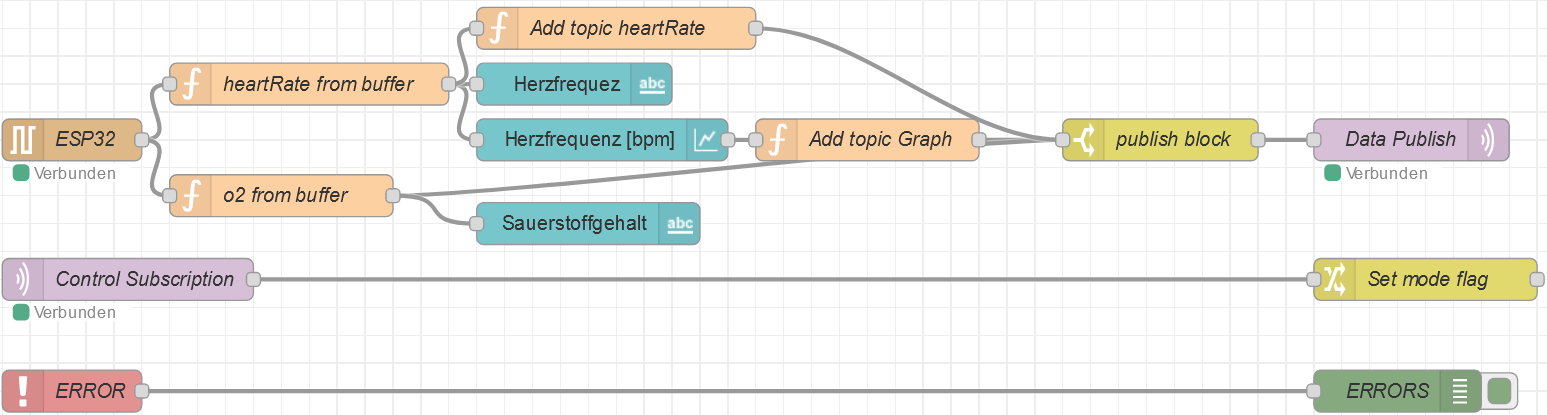
\includegraphics[width=0.9\textwidth]{node red flow}
  	\caption{Node-RED\cite{nodeRED} Datenfluss Darstellung}
  	\label{fig:nodeRedFlow}
  \end{figure}
	\subsubsection*{Serielle Schnittstelle}
	  Die serielle Schnittstelle ist so konfiguriert, dass sie mit einer Baudrate 115200 für 1000ms die Übertragung buffert und diese dann weitergibt. Dies geschieht im Knoten \quoteM{ESP32}.
	\subsubsection*{Verarbeitung des seriellen Inputs}
	  In den Knoten \quoteM{heartRate from buffer} und \quoteM{o2 from buffer} wird der serielle Mitschnitt jeweils aufgebrochen, die gesuchten Werte separiert und der Durchschnitt gebildet, um den Graph etwas zu glätten.
	  \begin{lstlisting}[language=JS, caption={Quellcode der Methode \quoteM{o2 from buffer} zum Lesen des Sauerstoffgehalts aus dem Buffer}, captionpos=b, label=srcO2]
	var o2 = 0.0;
	var i = 0;
	
	// split the serial protocol of 1 second into seperate messages.
	var words = msg.payload.split("\r\n");
	
	// seperate each message in single values for o2 and heartrate.
	words.forEach(function (item) {
		if(item.includes(";"))
		{
			var values = item.split(";");
			if(!isNaN(values[1]))
			{
				// add all valid o2 values and count them.
				o2 = parseFloat(o2) + parseFloat(values[1]);
				i = i + 1;
			}
		}
	});
	
	// return the average o2 value in payload.
	return [ {payload: o2 / i, topic: 2}];
	  \end{lstlisting}	
      Die Ausgabe dieser Methoden wird dann im Node-RED internen Dashboard als Absolutwerte und in Form eines Graphen für die Herzfrequenz visualisiert (Siehe Abbildung \ref{fig:nodeRedDashboard}). Das Graphen-Objekt wird im Datenfluss weitergegeben, um in der Android App weiterverwendet werden zu können.
      \begin{figure}[tph!]
      	\begin{center}
      		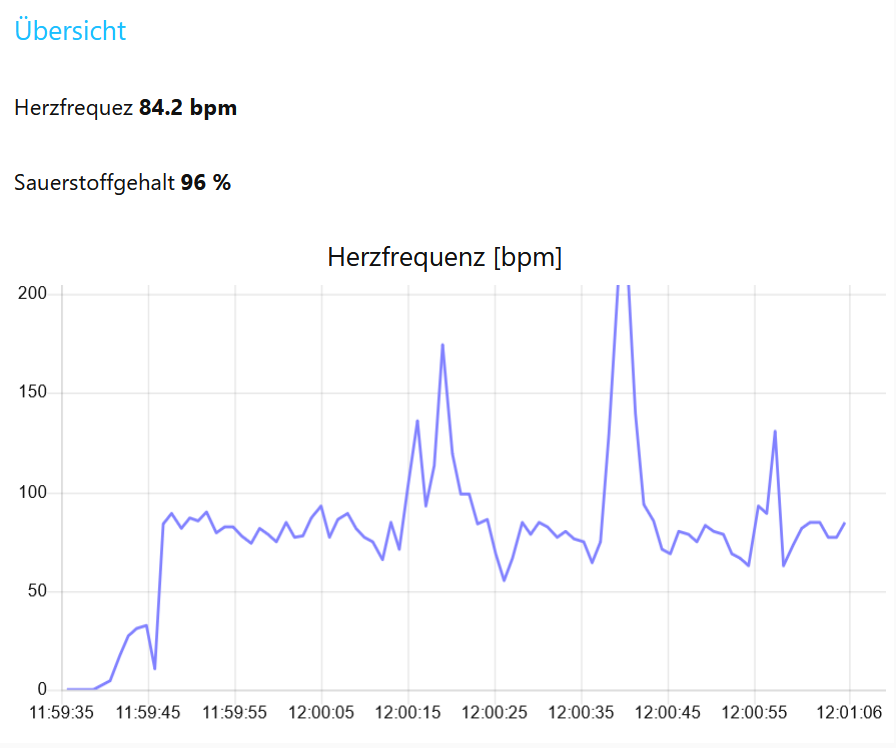
\includegraphics[width=0.5\textwidth]{node red dashboard}
	      	\caption{Node-RED Dashboard}
	      	\label{fig:nodeRedDashboard}
      	\end{center}
      \end{figure}\newpage
	\subsubsection*{MQTT Publishing}
  	  Im Anschluss daran werden die sogenannten Messages mit einem Topic, was dem in der Android App definierten Enumerate \quoteM{selectedView} entspricht.
	  \begin{lstlisting}[language=Java, caption={Quellcode des Enumerates \quoteM{selectedView} zur Auswahl der zu übertragenden Werte}, captionpos=b, label=srcSelectedView]
enum SelectedView
{
	heartRate,
	graph,
	o2
}
	  \end{lstlisting}
      In dem switch-Knoten \quoteM{publishBlock} werden dann nur die Messages, deren Topic Attribut der ID der ausgewählten Ansicht entsprechen, an den MQTT Publish Knoten weitergegeben. Dieser published dann die Werte an das Topic \quoteM{afkdcdjkcnks/sensor/data/raw/sensor}.
    \subsubsection*{Moduseinstellung}
      Der Knoten \quoteM{Control Subscription} abonniert das Topic \quoteM{afkdcdjkcnks/sensor/ctrl/raw/sensor}. Auf dieses published die Android Applikation die ID der ausgewählten Ansicht (Siehe Listing \ref{srcSelectedView}). Mit einem Abtastintervall von einer Sekunde wird der aktuelle Wert überprüft und im flow Context \quoteM{mode} gespeichert, auf welches dann der \quoteM{publish block Knoten} zugreift.	
  \subsection{Android Applikation}
  	  Die Android Applikation unterstützt Android Oreo oder höher. lässt sich im wesentlichen in drei Teile unterteilen. Das Frontend, das MQTT Modul und das Konfigurations-Lademodul.
  	  
  	  
  	  
  	  \subsubsection{Frontend}
  	    Die App besteht aus drei Views, jeweils eine für die in \ref{srcSelectedView} angebotenen Werte.
  	    
  	  	\begin{figure}[tph!]
  	  		\begin{center}
  	  			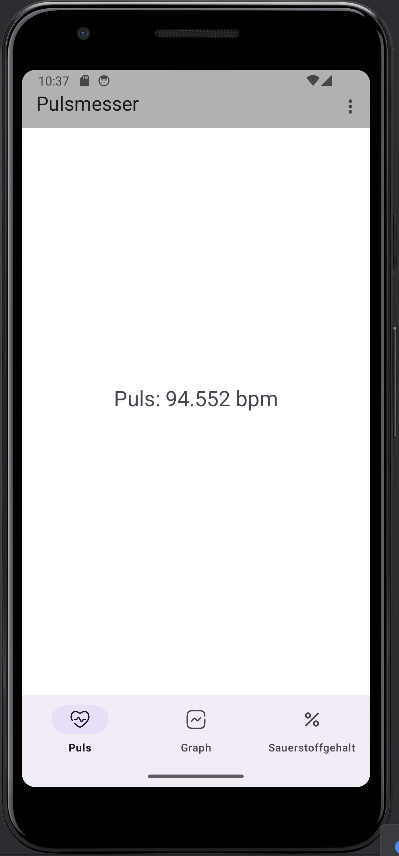
\includegraphics[height=6cm]{pulseview}
  	  			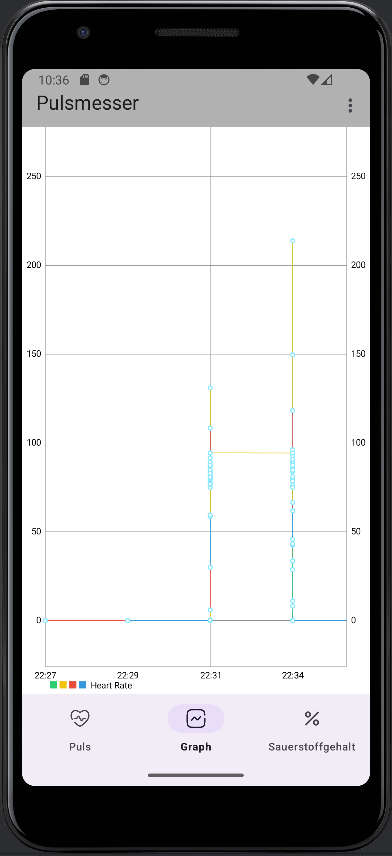
\includegraphics[height=6cm]{graph}
  	  			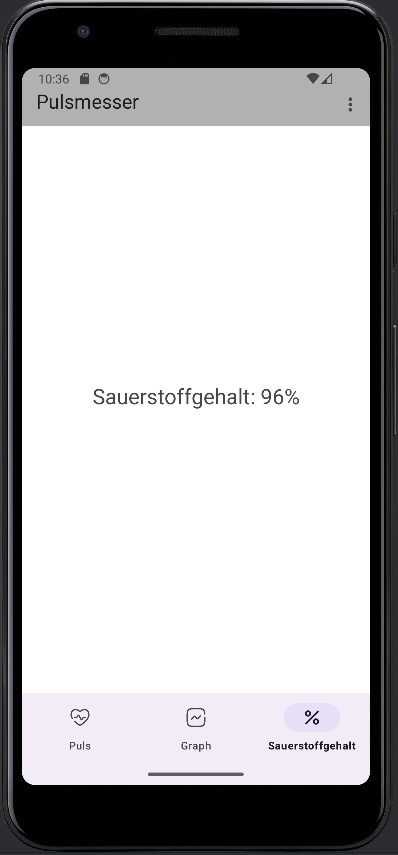
\includegraphics[height=6cm]{o2}
  	  			\caption{Die Views der Applikation}
  	  			\label{fig:pulseview}
  	  		\end{center}
  	  	\end{figure}
    	\paragraph{Pulsview}~\\
  	  	Hier wird der, vom Broker empfangene Puls als float-Zahl angezeigt. Zudem ertönt ein Herzschlag in Geschwindigkeit, die von dem erhaltenen Wert vorgegeben ist. Dieser lässt sich im Kontextmenü oben rechts ausschalten.
  	  
  \subsubsection{MQTT Schnittstelle}
   Die MQTT Schnittstelle besteht aus zwei Bereichen. Zuerst dem eigentlichen Client, der in Kapitel \ref{par:mqtt} näher beschrieben wird und dann dem Interface, welches zur Weitergabe der Nachrichten in der Applikation dient und in Kapitel \ref{par:isubscribe} erläutert ist.
   
   \paragraph{ISubscribe}~\\
   \label{par:isubscribe}
   Das MQTT Modul wurde mit der Paho Bibliothek der Eclipse Foundation\cite{paho_client} realisiert. Es ist eine statische Klasse, die nach Aufbau einer Verbindung zu einem MQTT-Broker bis zu drei Abonnenten vom Typ \quoteM{ISubscribe}.
   \begin{lstlisting}[language=Java, caption={Quellcode des Interfaces ISubscribe}, captionpos=b, label=srcISubscribe]
 	    	public interface ISubscribe {
 	    		void onMessageReceived(String message);
 	    		void unsubscribe();
 	    	}
   \end{lstlisting}
   Von diesen wird dann, sobald ein neuer Wert am Broker eingetroffen ist die Methode \quoteM{onMessageReceived} aufgerufen, mit dem Wert als Parameter. So werden die Daten automatisch in die Frontend Fragments geladen, sofern diese korrekt initialisiert sind.\par
   Die Methode \quoteM{unsubscribe} ist dazu da, explizit das Abonnement zu beenden und den Platz für ein anderes Fragment freizumachen. Sie wird in der Klasse \textbf{MainActivity} beim ändern des Tabs automatisch aufgerufen.
  	\paragraph{MqttModule}~\\
  	\label{par:mqtt}
		Die eigentliche MQTT Modulklasse hat folgende Methoden:\par
		\begin{figure}[tph!]
			\begin{tabularx}{\textwidth}{l l X}
				\textbf{Name} & \textbf{Parameter} & \textbf{Beschreibung}\\\hline
				\textbf{init} & String, String, & Füllt die Topic Attribute und den\\
				&  String & genutzten Klientnamen.\\\hline
				\textbf{isInit}&& Prüft ob alle in init gesetzten Parameter nicht leer sind.\\\hline
				\textbf{connect} & String, int & Baut eine TCP-Verbindung zum Broker auf mit URL und Port als Parameter.\\\hline
				\textbf{connect} & String, int, String, & Ruft init und connect auf.\\
				&  String, String &\\\hline
				\textbf{disconnect} && Baut die TCP-Verbindung zum Broker ab.\\\hline
				\textbf{publishCtrlMessage} & SelectedView & Published den Parameter als Integer an\\
				& (Listing \ref{srcSelectedView}) & den Broker.\\\hline
				\textbf{subscribeData} && Abonniert das angegebene DataTopic und setzt die Callbackmethode, dass in allen registrierten ISubscribe Objekten die onMessageReceived Methode aufgerufen wird.\\ \hline
				\textbf{addSubscription} & ISubscribe & Fügt Parameter zu Abonnenten hinzu, sofern ein Platz frei ist.\\\hline
				\textbf{removeSubscription} & ISubscribe & Entfernt Parameter aus Abonnenten, sofern er einer ist.\\
			\end{tabularx}
			\caption{Methoden der Klasse MqttModule}
		\end{figure}  		
  		Sie wird genutzt, indem beim Start der Anwendung der Client mit dem Broker verbunden wird und das Topic abonniert. Wenn sich das angezeigte Fragment ändert, wird dieses als Abonnent hinzugefügt, während das letzte entfernt wird. Zudem wird bei einem Wechsel ein Publish mit der neuen, ausgewählten View vollzogen.
  	  
  		
  		
  		
  		
  \subsection{\LaTeX{} Template Erweiterungen}
    \textbf{Erweitern der Inhaltsverzeichnistiefe}\\[0.3cm]
      Zur übersichtlicheren Aufschlüsselung wurde ein weiteres Level an Überschriften benötigt. Hierzu erweiterten wir unsere Dokumentenkonfiguration um folgenden Absatz, den wir von Stackexchange\cite{texTocDepth} übernahmen.
      \begin{lstlisting}[language=tex, caption={\LaTeX{} Quellcode zum Anzeigen einer vierten Inhaltsverzeichnisebene}, captionpos=b, label=srcTocDepth]
\setcounter{secnumdepth}{5}
\setcounter{tocdepth}{5}
\newcommand\simpleparagraph[1]{%
	\stepcounter{paragraph}\paragraph*{\theparagraph\quad{}#1}}
	 \end{lstlisting}
   	
	\textbf{Sprachsupport für JavaScript im listings-Paket}\\[0.3cm]
	  Um den Quellcode von Listing \ref{srcO2} ansprechend darstellen zu können wurde das von Prof. Dr. Schäfer gestellte \LaTeX{} Template erweitert um Quellcodesupport für JavaScript\cite{texJsInclusion}. Der dafür benötigte Quellcode wurde von Stackexchange übernommen und geringfügig verändert, um dem bestehenden Konzept zu entsprechen.
	  \begin{lstlisting}[language=tex, caption={\LaTeX{} Quellcode für JavaScript Support im Paket listings}, captionpos=b, label=srcJS]
\lstdefinelanguage{JS}{
	keywords={typeof, new, true, false, catch, function, return, null, catch, switch,
		      var, if, in, while, do, else, case, break},
	keywordstyle=\color{blue}\bfseries,
	ndkeywords={class, export, boolean, throw, implements, import, this},
	ndkeywordstyle=\color{blue}\bfseries,
	identifierstyle=\color{black},
	sensitive=false,
	comment=[l]{//},
	morecomment=[s]{/*}{*/},
	commentstyle=\color{battleshipgrey}\ttfamily,
	stringstyle=\color{cardinal}\ttfamily,
	morestring=[b]',
	morestring=[b]"
}
  	  \end{lstlisting}
	  
  %
  % Probleme und Diskussion
  %
  
  \section{Probleme und Diskussion}
	Die grö\ss ten Probleme bei der Implementation traten beim Umsetzen der MQTT Verbindungen auf. Der Zugriff auf ein persönliches HiveMQ Cluster von Node-RED ist selbst nach mehrstündiger Recherche nicht gelungen, weshalb wir probeweise auf den HiveMQ Public MQTT Broker gewechselt sind. Dies funktionierte auf Anhieb ohne Probleme.
  
  %
  % Zusammenfassung und Ausblick
  %
  
  \section{Zusammenfassung und Ausblick}
	Das Projekt ist als Konzept durchaus brauchbar für medizinische Anwendung. Man müsste nur die Alle Daten kontinuierlich zur Verfügung stellen. Sollte ein zuverlässigerer Puls und Sauserstoffgehalt Sensor eingebunden werden, der ESP\_32 eigenständig mit dem Broker kommunizieren und mit einem Token oder einer ID ausgestattet werden, könnte man das System komerziell einsetzen.\par
	So wäre es möglich, dass man über ein affiliate System Arztpraxen die Möglichkeit gibt, ihnen zugeordnete Geräte auszugeben, die der Patient nutzt. Durch diese Zuordnung könnte der Arzt vorbereitend auf eine Sprechstunde oder zur Ferndiagnose die gemessenen Werte online einsehen. \par
	Diese Idee ist zugegeben Datenschutztechnisch nicht auf Realisierbarkeit geprüft, könnte jedoch die Behandlung von chronischen Krankheiten, deren Symptomatik mit Blutwerten zusammenhängt modernisieren und da diese oft bei älteren, weniger mobilen Menschen auftreten vereinfachen.
  
  \clearpage 
  
  \listoffigures
  \lstlistoflistings
  
  \addcontentsline{toc}{section}{Literatur}
  \bibliographystyle{natdin}
  \bibliography{quellen}
  
%\include{anhang} % zum Beispiel hier die ChatGPT-Chatprotokolle einbinden (oder als extra-Datei)

\end{document}
